\section{Viola-Jones algoritam}

Kao primjer algoritama za detekciju objekata implementiran je i algoritam Viole i Jonesa opisan u poglavlju 3.2. Algoritam je implementiran korištenjem biblioteke \textit{OpenCV}.

Algoritam prima nekoliko ulaznih parametara od kojih je obavezan samo parametar "- -video" kojim se zadaje video na kojem da se vrši detekcija i praćenje osoba. Parametar "- -win-stride" je uređeni par vrijednosti $(x, y)$ koji određuje korak u smijeru $x$ i $y$ osi po kojima se kreće klizeći prozor. Zadana vrijednost je $(8, 8)$. Idući bitan parametar je "--scale". Ovaj parametar omogućuje detekciju ljudi različitih veličina na slici (i ljudi koji su blizu i ljudi koji su daleko). Povećanjem ovog parametra povećava se i rizik da ne budu detektirani svi objekti, ali istovremeno se algoritam i ubrzava. Obrnuto, smanjenjem ovog parametra algoritam detektira više objekata i usporava mu se rad. Posljedično, javlja se i više false-positiva. U implementaciji je ovaj algoritam postavljen na vrijednost $1.05$. Ostavljena je i mogućnost spremanja svake slike u videu (svakog \textit{framea}) parametrom "- -save" radi kasnije evaluacije. 

\begin{figure}[htp]
	\centering
	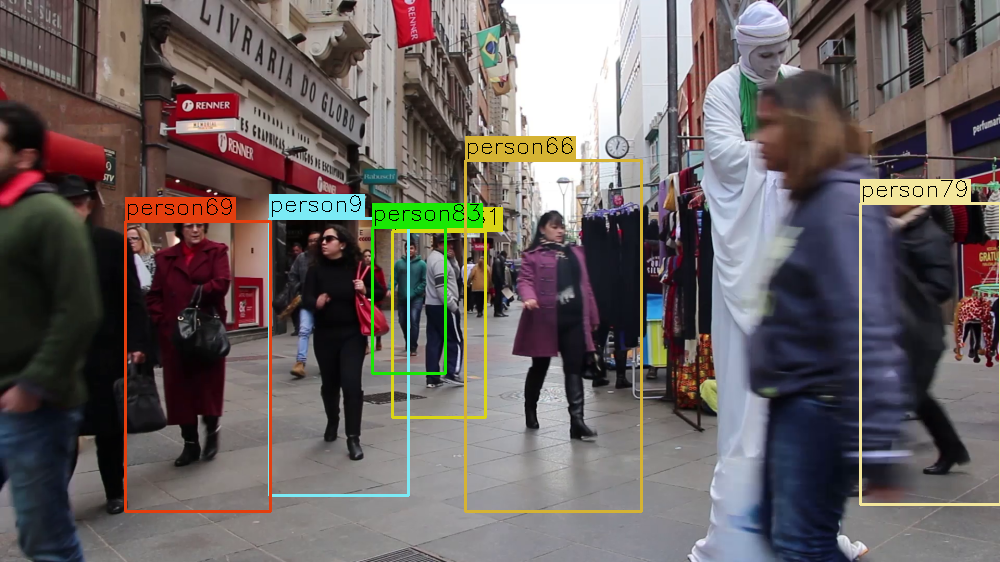
\includegraphics[width=9cm]{/home/luka/Workspaces/diplomski-rad/img/ViolaJonesFrames/frame_3.png}
	\caption{Primjer detekcije Viola-Jones algoritmom}
	\label{img:violaJones-detection-example}
\end{figure}

\section{YOLO}

U okviru ovog rada implementiran je i algoritam za detekciju objekata pod nazivom \textbf{YOLO - You Only Look Once} \citep{YOLO}. Ovaj algoritam je predvodnik novih revolucionarnih algoritama za detekciju objekata. Trenutno najnovija, treća, verzija ovog algoritma nastala je 2018. godine, dok se algoritam, u svojoj osnovnoj inačici, pojavio 2015. godine. Također, postoje dvije inačice svake verzije algoritma: \textit{full-YOLO} i \textit{tiny-YOLO}. Tiny-YOLO ima manju mrežu i, naravno, slabije sposobnosti, no ima bolje performanse. 

Prije ovog algoritma, detekcija objekata se vršila pomoću klasifikatorskih ili lokalizacijskih mreža. Takve mreže primjenjuju se na različita područja slike te na različito skaliranu sliku. One regije slike za koje su mreže vrlo sigurne smatraju se detekcijom. YOLO algoritam koristi potpuno novu paradigmu, novi pristup detekciji objekata. Ideja je da se kroz mrežu provuće jedna slika, bez skaliranja ili dovođenja različitih regija slike na ulaz mreže. Dakle, postupak detekcije objekata u mreži YOLO jest da mreža sama podijeli sliku na regije te predviđa okvire objekata (\textit{engl. bounding-box}) te njihove vjerojatnosti za svaku regiju. Odnosno, klasifikacija i lokalizacija objekata na slici te predviđanje okvira objekata su sve zadaće jedne mreže. 

\subsection{Dizajn i svojstva mreže}

U tablici \ref{tab:yolo_architecture} prikazana je arhitektura mreže Yolo. Radi preglednosti tablice, pod slojem Conv podrazumijeva se konvolucijski sloj dimenzija kako su napisane, Batch Normalization sloj koji, kako mu samo ime kaže, služi na normalizaciju \textit{batcha}, poboljšava konvergenciju modela dok istovremeno služi i kao regularizator. Na kraju je dodan i Leaky ReLu sloj.

\begin{minipage}{\linewidth}
\centering

\begin{tabular}{||l|l|l|l|l||}
\hline
	Ime sloja & Filteri & Korak & Dimenzije na ulazu & Dimenzije na izlazu \\
\hline
	Conv1 & 3 x 3 x 32 & 1 x 1 & 416 x 416 x   3 & 416 x 416 x  32 \\
\hline
	MaxPool1 & 2 x 2 & 2 x 2 & 416 x 416 x  32 & 208 x 208 x  32 \\
\hline
	Conv2 & 3 x 3 x 64 & 1 x 1 & 208 x 208 x  32 & 208 x 208 x  64 \\
\hline
	MaxPool2 & 2 x 2 & 2 x 2 & 208 x 208 x  64 & 104 x 104 x  64 \\
\hline
	Conv3 & 3 x 3 x 128 & 1 x 1 & 104 x 104 x  64 & 104 x 104 x 128 \\
\hline	
	Conv4 & 1 x 1 x 64 & 1 x 1 & 104 x 104 x 128 & 104 x 104 x  64 \\
\hline
	Conv5 & 3 x 3 x 128 & 1 x 1 & 104 x 104 x  64 & 104 x 104 x 128 \\
\hline
	MaxPool2 & 2 x 2 & 2 x 2 & 104 x 104 x 128 & 52 x  52 x 128 \\
\hline
	Conv6 & 3 x 3 x 256 & 1 x 1 & 52 x  52 x 128 & 52 x  52 x 256 \\
\hline
	Conv7 & 1 x 1 x 128 & 1 x 1 & 52 x  52 x 256 & 52 x  52 x 128 \\
\hline
	Conv8 &  3 x 3 x 256 & 1 x 1 & 52 x  52 x 128 & 52 x  52 x 256 \\
\hline
	MaxPool3 & 2 x 2 & 2 x 2 & 52 x  52 x 256 & 26 x  26 x 256 \\
\hline
	Conv9 & 3 x 3 x 512 & 1 x 1 & 26 x  26 x 256 & 26 x  26 x 512 \\
\hline
	Conv10 & 1 x 1 x 256 & 1 x 1 & 26 x  26 x 512 & 26 x  26 x 256 \\
\hline
	Conv11 & 3 x 3 x 512 & 1 x 1 & 26 x  26 x 256 & 26 x  26 x 512\\
\hline
	Conv12 & 1 x 1 x 256 & 1 x 1 & 26 x  26 x 512 & 26 x  26 x 256 \\
\hline
	Conv13 & 3 x 3 x 512 & 1 x 1 & 26 x  26 x 256 & 26 x  26 x 512 \\
\hline
	MaxPool4 & 2 x 2 & 2 x 2 & 26 x  26 x 512 & 13 x  13 x 512 \\
\hline
	Conv14 & 3 x 3 x 1024 & 1 x 1 & 13 x  13 x 512 & 13 x  13 x 1024 \\
\hline
	Conv15 & 1 x 1 x 512 & 1 x 1 & 13 x  13 x 1024 & 13 x  13 x 512 \\
\hline
	Conv16 & 3 x 3 x 1024 & 1 x 1 & 13 x  13 x 512 & 13 x  13 x 1024 \\
\hline
	Conv17 & 1 x 1 x 512 & 1 x 1 & 13 x  13 x 1024 & 13 x  13 x 512 \\
\hline
	Conv18 & 3 x 3 x 1024 & 1 x 1 & 13 x  13 x 512 & 13 x  13 x 1024 \\
\hline
	Conv19 & 3 x 3 x 1024 & 1 x 1 & 13 x  13 x 1024 & 13 x  13 x 1024 \\
\hline
	Conv20 & 3 x 3 x 1024 & 1 x 1 & 13 x  13 x 1024 & 13 x  13 x 1024 \\
\hline
\hline
	Route & from & Conv13 & & \\
\hline
	Conv21 & 1 x 1 x 64 & 1 x 1 & 26 x  26 x 512 & 26 x  26 x  64 \\
\hline
\hline
	Space2Depth & reshape & & & \\
\hline
	Concatenate & Route from Conv20 & and & Space2Depth & \\
\hline
	Conv22 & 3 x 3 x 1024 & 1 x 1 & 13 x  13 x 1280 & 13 x  13 x 1024 \\
\hline
	Conv23 & 1 x 1 x 425 & 1 x 1 & 13 x  13 x 1024 & 13 x  13 x 425 \\
\hline
\hline
\end{tabular}
\captionof{table}{Yolo arhitektura} \label{tab:yolo_architecture} 
\end{minipage}

\subsection{Podjela slike}
\label{cells-section}

Kada se na ulaz mreže dovede slika, prva stvar koju mreža napravi jest da podijeli sliku u \textbf{C} x \textbf{C} ćelija kao što to prikazuje slika \ref{img:yolo_grid_cells}. Svaka od tih ćelija predviđa točno \textbf{jedan} objekt. Primjerice, žuta ćelija na slici pokušava predvidjeti objekt klase osoba čiji se centar (plava točka na slici desno) nalazi unutar te čelije.

\begin{figure}[htp]
	\centering
	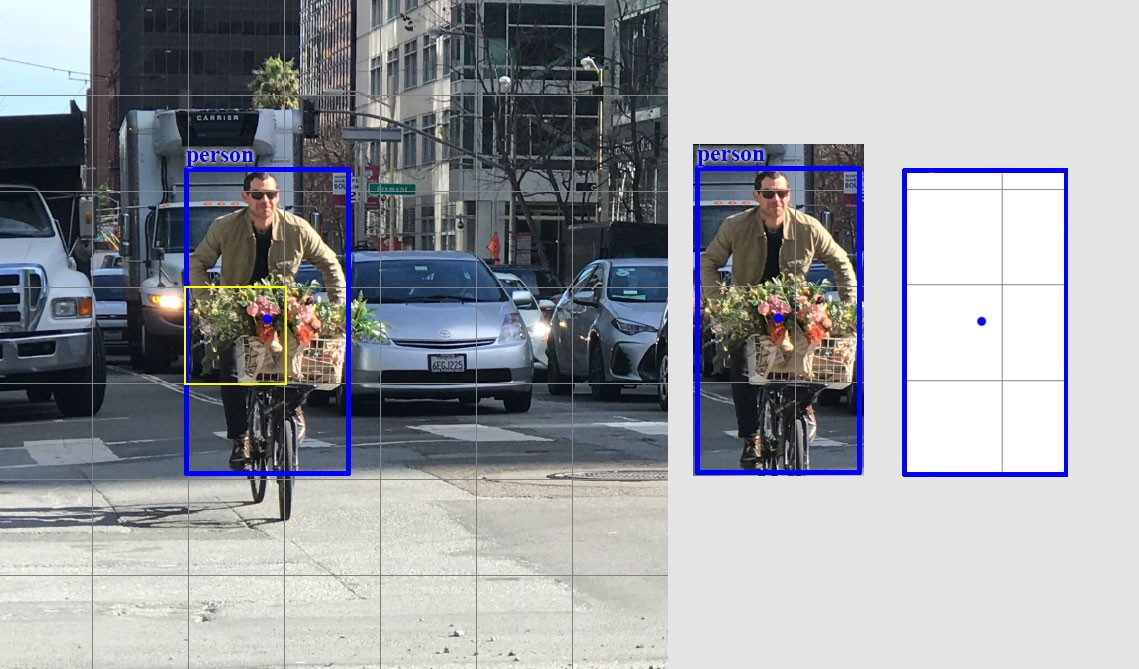
\includegraphics[width=10cm]{/home/luka/Workspaces/diplomski-rad/img/Yolo_grid.jpeg}
	\caption{Podijela slike na \textbf{C} x \textbf{C} ćelija}
	\label{img:yolo_grid_cells}
\end{figure}

Svaka ćelija predviđa fiksan broj okvira (\textit{engl. bounding boxes}. Na slici \ref{img:bounding_boxes} žuta ćelija predviđa dva okvira kako bi locirala osobu na slici. 

\begin{figure}[htp]
\centering
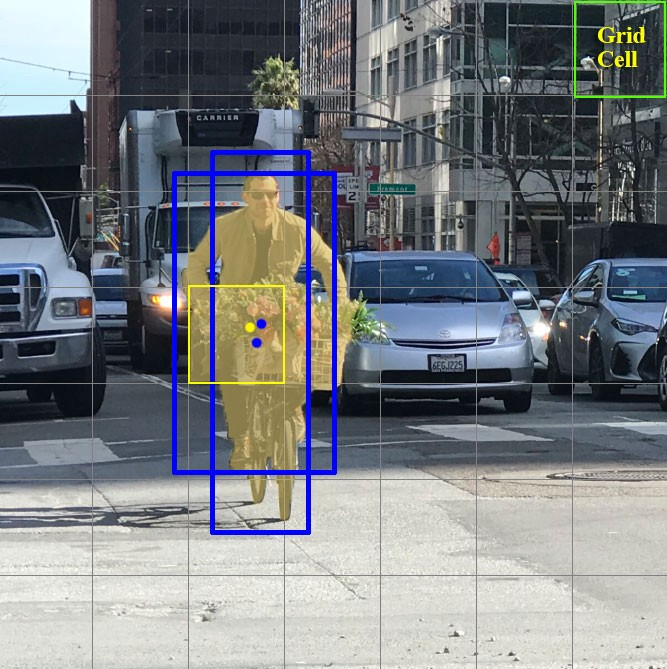
\includegraphics[width=10cm]{/home/luka/Workspaces/diplomski-rad/img/Yolo_cell_boxes.jpeg}
\caption{Predviđanje okvira}
\label{img:bounding_boxes}
\end{figure}

Međutim, mogućnost predviđanja samo jednog objekta po čeliji donekle ograničava algoritam u smislu blizine objekata koje može detektirati. Odnosno, ako se u čeliji nalazi više od 1 objekta, algoritam mora odabrati samo 1 koji od njih koji će detektirati.  

Za svaku čeliju \textbf{C} algoritam predviđa:
\begin{itemize}
	\item \textbf{B} okvira te za svaki okvir njegovu pouzadnost (\textit{engl. box confidence score})
	\item samo jedan objekt
	\item \textbf{P} vjerojatnosti, po jednu za svaku klasu \textbf{C}
\end{itemize}

Ulaz u mrežu može biti proizvoljne veličine, no mreža YOLO preoblikuje ulaz u dimenzije $416\times416\times3$ kako bi ga mogao dovesti na ulaz u mrežu. Mreža dijeli sliku na $13\times13$ ćelija. Svaka ćelija predviđa 5 okvira za objekt koji se nalazi u toj čeliji (ako se nalazi), te svaki od okvira ima 85 parametara. Izlaz iz mreže je oblika $(13, 13, 425)$. U svrhu razumijevanja izlaza iz mreže, zgodno ga je zamisliti kao kompozit tri tenzora:

\begin{itemize}
	\item pouzdanost okvira \textit{(engl. box\_confidence)} kao tenzor dimenzije $(13\times13, 5, 1)$ koji sadrži $p_c$ pouzdanost postojanja objekta u svakom od 5 predviđenih okvira u čeliji \textbf{C} za svaku od $13\times13$ ćelija
	\item okviri \textit{(engl. boxes)} kao tenzor dimenzije $(13\times13, 5, 4)$ koji sadrži $(x_{top}, y_{top}, x_{bottom}, y_{bottom})$ za svaki od 5 okvira u čeliji
	\item vjerojatnosti klasa za okvire \textit{(engl. box\_class\_prob)} kao tenzor dimenzije $(13\times13, 5, 80)$ koji čuva informaciju o pouzdanosti za svaku od 80 klasa za svaki od 5 okvira u čeliji.
\end{itemize}

\begin{figure}[htp]
	\centering
	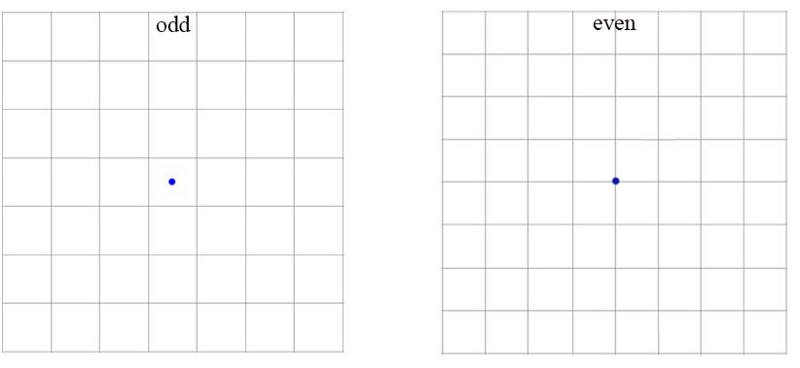
\includegraphics[width=8 cm]{/home/luka/Workspaces/diplomski-rad/img/yolo_grid.jpeg}
	\caption{Neparan i paran broj ćelija po dimenziji}
	\label{img:yolo-grid}
\end{figure}

Kao što prikazuje slika \ref{img:yolo-grid}, neparan broj ćelija po dimenziji (npr. $13\times13$) je pogodan jer je jednostavnije odrediti u kojoj se čeliji objekt nalazi.

\subsection{Funkcija gubitka}

Yolo algoritam predviđa više okvira po jendoj čeliji na slici. Od svih tih ćelija, potrebno je zadržati samo one u kojima se zaista nalazi objekt. U tu svrhu, izabire se ona ćelija koja ima naveći IoU (\textit{engl. Intersection over Union}) sa stvarnim objektom (\textit{engl. ground truth}). Za računanje gubitka, Yolo koristi sumu kvadrata pogrešaka predviđanja algoritma i stvarnih objekata. Zbog ideje Yolo algoritma da se klasifikacija i lokalizacija rade istom mrežom u jednom prolasku, funkcija gubitka sastavljena je od nekoliko dijelova.

\begin{figure}[htp]
	\centering
	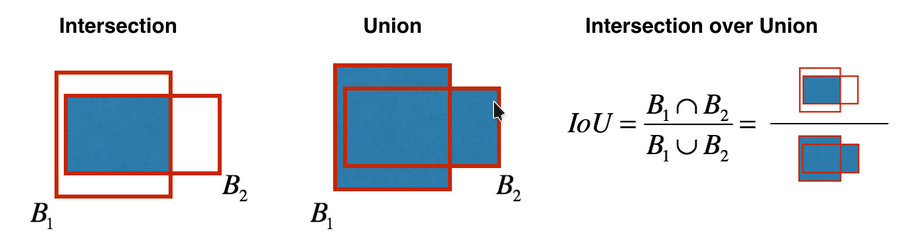
\includegraphics[width=11cm]{/home/luka/Workspaces/diplomski-rad/img/IoU.png}
	\caption{Intersection over union}
	\label{img:IoU}
\end{figure}

\begin{itemize}
	\item{\textbf{Pogreška klasifikacije}}
	
	Ako je objekt detektiran, pogreška klasifikacije u svakoj čeliji računa se kao kvadrat pogreške uvjetne vjerojatnosti za svaku klasu.
	
	\begin{equation}
		\centering
		\sum_{i=1}^{S\times S} 1_i^{obj} \sum_{c \in klase} (p_i(c) - \hat{p}_i(c))^2
		\label{eq:classification-loss}
	\end{equation}
	
	gdje 
	\begin{itemize}
		\item $1_i^{obj} = 1$ ako se objekt pojavljuje u čeliji i, inače $0$
		\item $\hat{p}_i(c)$ označava uvjetnu vjerojatnost klase $c$ u čeliji $i$
	\end{itemize}
	
	\item{\textbf{Pogreška lokalizacije}}
	
	Ovaj segment funkcije pogreške mjeri grešku u lokaciji i veličini predviđenih okvira. U obzir se uzimaju samo oni okviri u kojima se objekt nalazi. Ideja je da se jednaka greška u velikom i u malom predviđenom okviru ne kažnjavaju jednako (npr. greška od 2px u velikom i malom okviru). Zbog toga Yolo predviđa \textbf{korjene kvadrata} visine i širine okvira. Nadalje, kako bi još točije predviđao okvire, pogreška okvira se množi paramterom $\lambda_{coord}$.
	
	\begin{align}
		\centering
		\begin{split}
			\lambda_{coord}\sum_{i=0}^{S^2}\sum_{j=0}^{B} 1_{ij}^{obj} [(x_i - \hat{x}_i)^2 + (y_i - \hat{y}_i)^2] + \\
			\lambda_{coord}\sum_{i=0}^{S^2}\sum_{j=0}^{B} 1_{ij}^{obj} [(\sqrt{w_i} - \sqrt{\hat{w}_i})^2 + (\sqrt{h_i} - \sqrt{\hat{h}_i})^2]
		\end{split}
		\label{eq:localization-loss}
	\end{align}
	
	gdje 
	\begin{itemize}
		\item $1_{ij}^{obj} = 1$ ako se objekt nalazi u $j$-tom okviru $i$-te ćelije, inače $0$
		\item $\lambda_{coord}$ parametar za ugađanje težine za pogrešku u koordinatama okvira
	\end{itemize}
	
	\item{\textbf{Pogreška pouzdanosti}}

	Ovdje se javljaju dva slučaja:
	\begin{enumerate}
		\item \textbf{Objekt je detektiran u okviru}
		
		\begin{equation}
			\centering
			\sum_{i=0}^{S^2}\sum_{j=0}^{B} 1_{ij}^{obj} (C_i - \hat{C}_i)^2
			\label{eq:confidence-loss-1}
		\end{equation}
		
		gdje 
		\begin{itemize}
			\item $1_{ij}^{obj} = 1$ ako se objekt nalazi u $j$-tom okviru $i$-te ćelije, inače $0$
			\item $\hat{C}_i$ jest iznos pouzdanosti za okvir $j$ u čeliji $i$
		\end{itemize}
		
		\item \textbf{Objekt nije detektiran u okviru}
		
		Večina okvira ne sadrži objekt što dovodi do problema neravnomjernosti klasa, odnosno, model se trenira da puno češće detektira pozadinu nego sami objekt. Kako bi se ovaj problem riješio, gubitak se množi faktorom $\lambda_{no-obj}$ koji ima vrijednost između $0$ i $1$.
		
		\begin{equation}
			\centering
			\lambda_{no-obj}\sum_{i=0}^{S^2}\sum_{j=0}^{B} 1_{ij}^{no-obj} (C_i - \hat{C}_i)^2
			\label{eq:confidence-loss-2}
		\end{equation}
		
		gdje 
		\begin{itemize}
			\item $1_{ij}^{no-obj}$ jest komplement gornjeg izraza $1_{ij}^{obj}$
			\item $\hat{C}_i$ jest iznos pouzdanosti za okvir $j$ u čeliji $i$
			\item $\lambda_{no-obj}$ je faktor kojim se smanjuje iznos gubitka pri detekciji pozadine
		\end{itemize}
		
	\end{enumerate}	
		
\end{itemize}

\subsection{Anchor boxes}
\label{anchor-boxes-section}

\begin{figure}[htp]
	\centering
	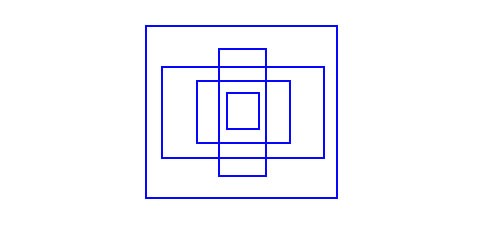
\includegraphics[width=8cm]{/home/luka/Workspaces/diplomski-rad/img/Anchor_boxes_img.jpeg}
	\caption{Klasteri dimenzija za anchor boxeve}
	\label{img:anchor-boxes}
\end{figure}

\textit{Anchor boxes} ili \textit{priors} jest još jedan pojam uveden ovim algoritmom. Kako u početku treninga mreža ne bi predviđala okvire nasumično, predloženo je da se, ovisno o domeni i podacima, izabere $n$ najčešćih okvira koji najbolje opisuju klase u tom skupu podataka. Primjerice, pješake se uglavnom može označiti uspravnim pravokutnim okvirom, dok je kod automobila okvir obično polegnuti pravokutnik. Na ovaj način uzeto je 5 standardnih okvira (\textit{anchor boxes}) koji su izračunati K-means klusteringom ($k=5$) iz COCO i VOC2007 skupova podataka kako bi se pronašle centoride $k$ najboljih klastera. Da bi se odredile točne dimenzije standardnih okvira, korišena je IoU mjera. Izračunati anchor boxevi prikazani su slikom \ref{img:yolo-anchors}. Ljubičasti okviri uzeti su iz COCO skupa podataka, a bijeli sa crnim rubom iz VOC2007 skupa podataka.

\begin{figure}[htp]
	\centering
	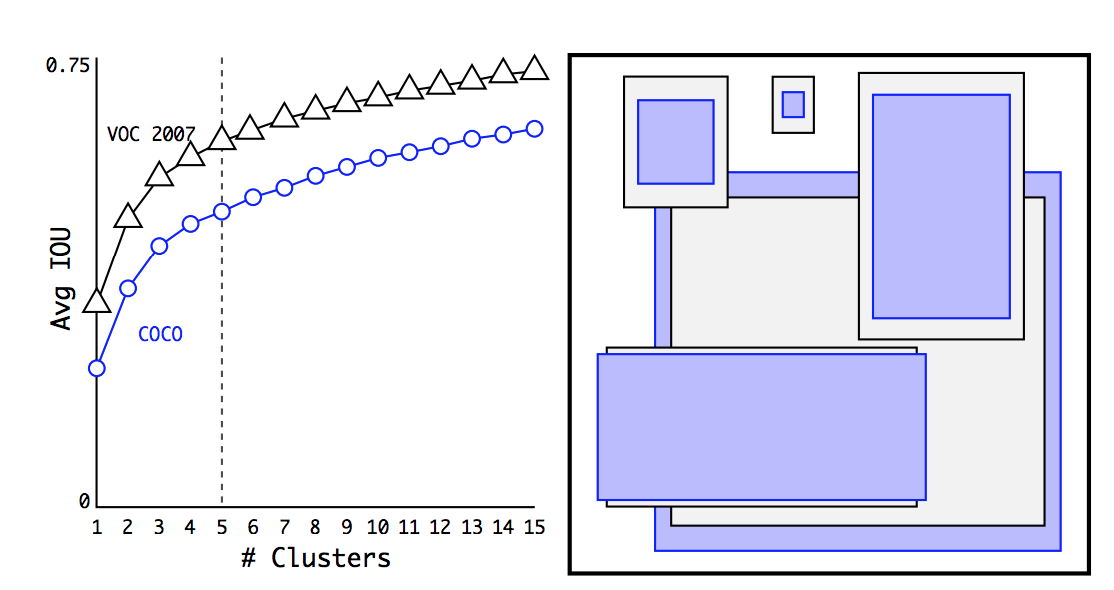
\includegraphics[width=9cm]{/home/luka/Workspaces/diplomski-rad/img/Yolo_anchor_boxes.png}
	\caption{Standardni okviri dobiveni K-means klasteringom i IoU mjerom \citep{YOLO}}
	\label{img:yolo-anchors}
\end{figure}

Tako sada Yolo mreža predviđa koordinate okvira objekta direktno, no relativno u odnosu na pozicuju promatrane ćelije od gornjeg lijevog ruba. Nadalje, okviri se predviđaju kao odstupanje od nekog od standardnih okvira. To odstupanje je ograničeno kako nebi bilo koji okvir mogao prijeći u bilo koji drugi jer se onda gubi smisao ovog cijelog postupka. Ograničavanjem odstupanja omogućeno je kako bi se svako predviđanje moglo opredjeliti za točno jedan oblik iz skupa standardnih okvira.

\subsection{Backbone}

Mreža kojom se inicijalizira Yolo mreža naziva se \textit{DarkNet} \citep{Darknet}. Mreža je prikazana na slici \ref{img:darknet}

\begin{figure}[htp]
	\centering
	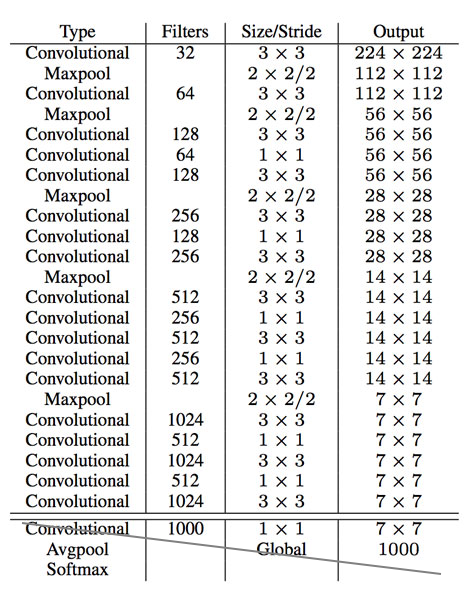
\includegraphics[width=8cm]{/home/luka/Workspaces/diplomski-rad/img/Darknet.png}
	\caption{Originalna DarkNet-19 mreža \citep{YOLO}}
	\label{img:darknet}
\end{figure}

Zadnji slojevi (koji su prekriženi na slici \ref{img:darknet}) izbačeni su za potrebe Yolo mreže. Ova arhitektura zahtjeva oko 5.8 milijardi operacija što je, u usporedbi sa VGG16 mrežom koja ima 3 sloja manje i zahtjeva oko 30.69 milijardi operacija za samo jednu sliku veličine $224 \times 224$, izuzetno malo i efikasno.

\subsection{Trening}

Prvo se trenira mreža DarkNet-19 za klasifikaciju na ImageNet skupu podataka sa 1000 klasa objekata u 160 epoha koristeći stohastički gradijentni spust (\textit{SGD}). Stopa učenja inicijalno je postavljena na vrijednost $0.1$ sa polinomijalnim raspadom potencije $4$, \textit{weight decay} parametrom postavljenim na $0.0005$ te momentom vrijednosti $0.9$. Tijekom treninga koriste se standardne metode izmjene podataka kao što su nasumično izrezivanje, rotacija i izmjene boje.

Zatim se izgradi mreža YOLO, prenesu se težine iz DarkNet mreže u početne slojeve mreže YOLO, te se ponovo trenira. Stopa učenja kreće od vrijednosti $10^{-3}$, a smanjuje se nakon 10, 60 i 90 epoha na isti način kao i kod treniranja DarkNeta. Parametar \textit{weight decay} postavljen je na vrijednost od $0.0005$, a moment na vrijednost $0.9$. Koriste se i metode izmjene boja, nasumičnog izrezivanja itd. kako bi algoritam bio što robusniji. Mreža se na taj način trenira na COCO i VOC2007 skupovima podataka.

Yolo mreža može primati slike različitih veličina. Svakih 10 \textit{batcheva} algoritam nasumično odabere neku veličinu slike za treniranje modela (veličina slike mora biti višekratnik broja $32$). Na taj način, prisiljava se mrežu da predviđa dobro za slike različitih dimenzija i skala. Na taj način omogućava se prilagodba mreže za određenu svrhu. Primjerice, ako je potrebno raditi predviđanja u stvarnom vremenu, moguće je davati manje slike algoritmu kako bi predviđanja bila brža. Ako je pak cilj da predviđanja budu što točnija, mogu se uzimati slike veće rezolucije.

\subsection{Predviđanje}

Način na koji YOLO detektira objekte i predviđa okvire objašnjeni su u podpoglavljima \ref{cells-section} i \ref{anchor-boxes-section}. No još nije spomenuto na koji način YOLO zaključuje koje okvire treba odbaciti a koje zadržati. Dakle, za neki objekt mreža predvidi nekoliko okvira. Metoda kojom se odabiru okviri za odbacivanje naziva se \textbf{Non-Maximal Suppression}. Način na koji ta metoda radi jest da poreda okvire po pouzdanosti, iterira kroz njih i odbacuje sve okvire koji predviđaju istu klasu kao neki od prethodnih i imaju IoU veći od $0.5$ sa tim prethodnim okvirom iste klase. Taj proces se ponavlja dok svi okviri ne budu ili odbačeni ili zadržani.

\begin{figure}[htp]
	\centering
	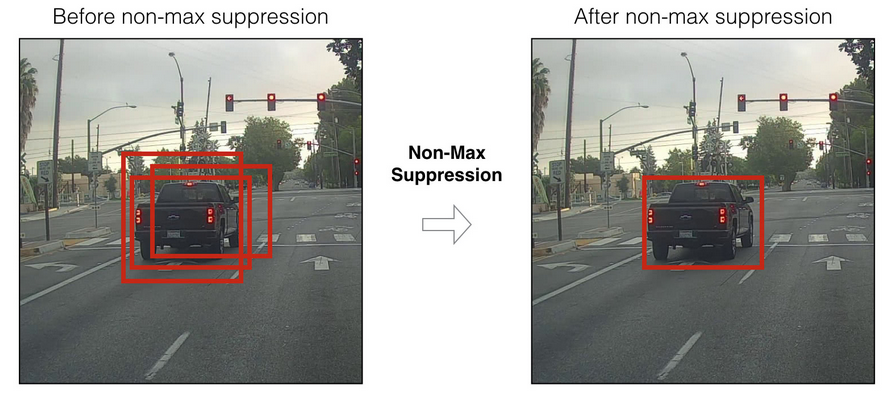
\includegraphics[width=10cm]{/home/luka/Workspaces/diplomski-rad/img/NMS.png}
	\caption{Non-Maximal Suppression}
	\label{img:nms}
\end{figure}